\documentclass{article}

\usepackage{amsfonts}
\usepackage{amsmath}
% \usepackage{svg} %For including svgs
% \svgpath{{../assets/}}
\usepackage{graphicx}
\graphicspath{ {../assets/} }
\usepackage[margin=1in]{geometry} %Change margins
\usepackage{hyperref} %For hyperlinks in table of contents and other
\usepackage{float} %For using H in figure
\usepackage{subcaption} %For subfigures
\usepackage{booktabs} %For tables
\usepackage{multirow} %For tables

%\usepackage[charsperline=120]{jlcode} %For Julia Code Listing https://github.com/wg030/jlcode

\addtolength{\jot}{1em} %https://tex.stackexchange.com/questions/14679/amsmath-align-environment-row-spacing

\title{Optimization Assignment 3\\Linear Programs and Applications}
\date{Winter 2021}
\author{Kim Paolo Laberinto (7771083)}

\begin{document}
    \maketitle
    \newpage

    \tableofcontents
    \newpage


    \section{Q1. Linear Programming Applied to Diet Optimizaton}

    \section{Q2. Example of Conversion to Standard Form}

    \section{Q3. Example of Graphically Solving a Linear Program}

    \begin{figure}[H]
        \centering
        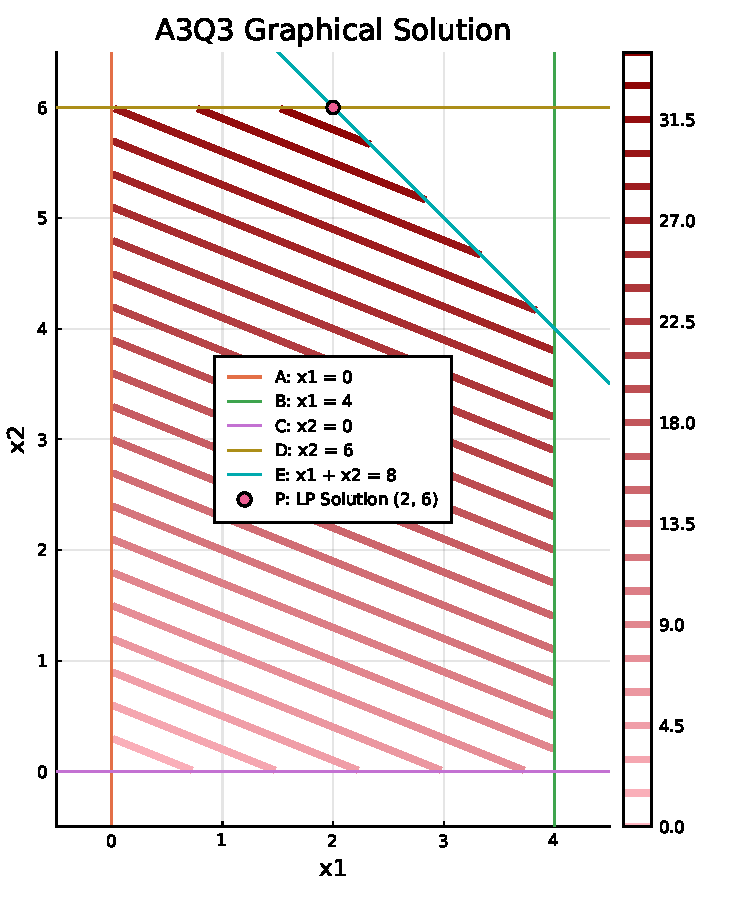
\includegraphics[width=0.5\linewidth]{A3Q3_Plot.pdf}
        \caption{Graphical Solution to A3Q3 question, showing feasible region, objective contours, and solution.}
        \label{fig:A3Q3_GraphicalSolution}
    \end{figure}

    \section{Q4. Textbook Questions}

    \subsection{12.9}

    \subsection{12.15}

    \subsection{12.21}

    \subsection{12.22}


    \newpage
    \appendix

    \section{Source Code}

\end{document}